\documentclass[11pt]{article}
\usepackage{fullpage}
\usepackage{amsmath}
\usepackage{graphicx}
\usepackage{graphics}
\usepackage{hyperref}
\usepackage[english]{babel}
\usepackage{verbatim}
\usepackage[T1]{fontenc}
\usepackage{tikz,overpic}
\usetikzlibrary{fit,shapes.misc}

\def\No{\textsf{N}}
\def\Ga{\textsf{Ga}}
\def\BF{\textit{BF}}
\def\n0{n_0}
\newcommand{\St}{\textsf{t}}
\newcommand{\E}{\textsf{E}}

\def\data{\text{data}}
\newcommand{\iid}{\ensuremath{\mathrel{\mathop{\sim}\limits^{\rm iid}}}}
\def\handwriting{\fontencoding{T1}\fontfamily{augie}\selectfont}

\title{Optional Reading:\\ Derivations for comparing two paired means using Bayes factors}

\author{Dr.~Merlise Clyde}
\date{}


\usepackage{Sweave}
\begin{document}
\Sconcordance{concordance:4-3-2-pair-notes.tex:4-3-2-pair-notes.Rnw:%
1 29 1 1 0 6 1 1 6 11 1 1 6 3 1 1 2 17 0 1 2 4 1 1 14 1 2 233 1}



\maketitle


\begin{Schunk}
\begin{Sinput}
> myblue = rgb(86,155,189, name="myblue", max=256)
> mydarkgrey = rgb(.5,.5,.5, name="mydarkgrey", max=1)
> par(mar=c(5, 9, 2, 2), col.lab=mydarkgrey, col.axis=mydarkgrey, col=mydarkgrey)
\end{Sinput}
\end{Schunk}



%\begin{beamercolorbox}[rounded=true,shadow=true,wd=.9\textwidth]{ExBox}
%A SurveyUSA poll on parents perceptions of bullying of their children
%\end{beamercolorbox}



\section*{Paired Data}
In the example in the video,  we have $n = 10$ paired observations $Y_{iB}$ and $Y_{iS}$  for $i = 1, \ldots, n$ representing the concentrations of zinc at the bottom and surface, respectively.



Rather than working with the two groups of observations, we will work with the differences $D_{i} \equiv Y_{iB} - Y_{iS}$ to make inference about the difference in the means $\mu_1 - \mu_2 \equiv \mu$ converting this problem to a one group Normal problem.   

\begin{Schunk}
\begin{Sinput}
> zinc
\end{Sinput}
\begin{Soutput}
   bottom surface difference
1   0.430   0.415      0.015
2   0.266   0.238      0.028
3   0.567   0.390      0.177
4   0.531   0.410      0.121
5   0.707   0.605      0.102
6   0.716   0.609      0.107
7   0.651   0.632      0.019
8   0.589   0.523      0.066
9   0.469   0.411      0.058
10  0.723   0.612      0.111
\end{Soutput}
\end{Schunk}

We will make the same assumptions about the distributions of the differences as in the case of the frequentist paired t-test.  That is conditional on the parameters $\mu$ and $\sigma^2$
the observed differences are independently and identically distributed from a  normal distribution expressed notationally as
$$D_i \mid \mu, \sigma^2 \iid \No(\mu, \sigma^2)$$.  To check the assumption of normality we can look at a histogram or normal quantile plot of the sampled differences. 

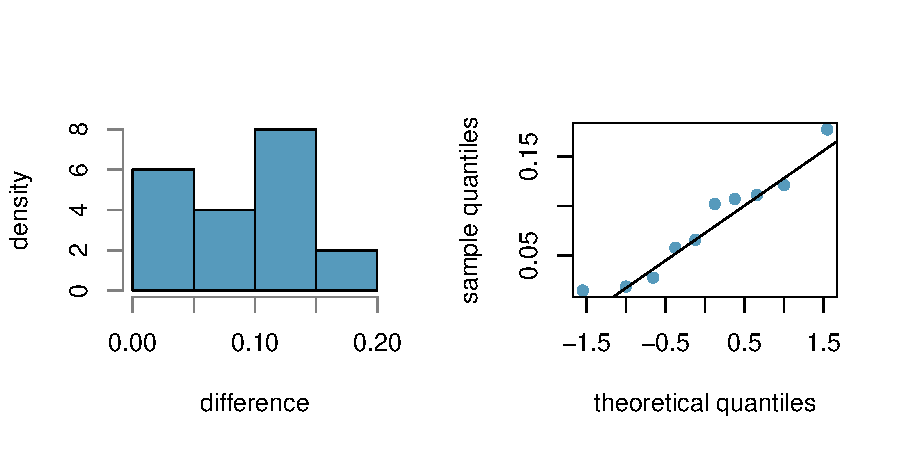
\includegraphics{4-3-2-pair-notes-hist}

\subsection*{Likelihood}
The normal sampling model leads to a likelihood function 
$$
{\cal{L}}(\mu, \sigma^2) = \prod_{i = 1}^{n} \frac{1}{\sqrt{\sigma^2 2 \pi}} \exp{\left( - \frac{1}{2}\frac{(D_i - \mu)^2}{\sigma^2} \right)} 
$$
where the likelihood function is proportional to the sampling distribution of the data.
To simplify our calculations we can reduce the data down to two "sufficent" statistics, where
$$ \bar{D} \mid \mu, \sigma^2 \sim \No(\mu,  \sigma^2/n)$$
and is independent of 
$$ 
s^2 \mid \sigma^2 \sim  \Ga\left(\frac{n - 1}{2},  \frac{n-1}{2 \sigma^2}\right)
$$
where $s^2$ is the sample variance, $s^2 = \sum(D_i - \bar{D})^2/(n-1)$, and $\Ga$ is a gamma distribution.  Note, we will use the rate parameterization of the gamma, so if $Y \sim \Ga(a, b)$ then $Y$ has a probability density function 
$$
p(y) = \frac{1}{\Gamma(a)} b^a y^{a - 1} e^{- y b} 
$$
with expected value $a/b$.  From this we can see that $\E[s^2] = \sigma^2$ so that the sample variance is an unbiased estmator of the population variance. {\it Note that the rate parameterization that we are using here is different from the scale parameterization that is used in Week 2 for the Conjugate Poisson-Gamma}.  The rate parameterization leads to easier updating rules as we will see.   


For ease of derivation, we are going to create a new parameter $\phi \equiv 1/\sigma^2$ to help with specifing a conjugate prior distribution.  The paramter $\phi$ is known as the precision;  if the variance is small we have high precision, while if the variance is small we have more uncertainty  and low precision.  In the new parameterization our two statistics have sampling distibutions

\begin{align}
 \bar{D} \mid \mu, \phi & \sim \No\left(\mu,  1/(\phi n)\right) \\
 s^2_d \mid \phi & \sim  \Ga(\nu/2,  \nu \phi/2 )
\end{align}
where $\nu = n-1 $ is the usual degrees of freedom leading to a likelood function based on taking the product of the independent distributions 
$$
{\cal{L}}(\mu, \phi) \propto (n\phi)^{1/2} \frac{1}{\sqrt{(2 \pi)}} 
\exp\left\{- \frac 1 2  n \phi (\bar{D} - \mu)^2 \right\}
\frac{1 }{\Gamma(\nu/2)} \left(\frac{\nu \phi}{2}\right)^{\nu/2} {s^2_d}^{\nu/2 - 1} \exp{- \frac{\phi \nu s^2_d}{2}}.
$$

Note:  you could just start with the independent normal samples and through some algebra rearrange to get to this.

\section*{Conjugate Normal-Gamma Prior Distribution}


For Bayesian inference we need to assign prior distributions to all of the unknown parameters under all hypotheses. As a first attempt, conjugate prior distributions are a convenient choice or as we will encounter later provide building blocks for more complex distributions. Recall a conjugate prior distribution is one where the posterior distribution and the prior distribution are in the same family. 

\subsection*{Conjugate Prior and Posterior for $\mu$ given $\phi$}

In Week 2 we studied the conjugate prior for a normal mean assuming that $\sigma^2$ or $\phi$ was known.   While in this case the variance is unknown, 
conditional on $\sigma^2$ (or $\phi$ now), the conjugate prior for $\mu$ given $\phi$ is a normal distribution,  
$$ \mu \mid \phi \sim \No \left(m_0, \frac{1}{n_0 \phi} \right)
$$
where $m_0$ is the prior mean and $n_0$ is a hyperparameter that is used to represent
how concentrated or less concentrated the distribution is about $m_0$ relative to the precision $\phi$, and may be
thought of as a prior imaginary sample size upon which the prior distribution is 
based if there are no historical observations. Taking $n_0 = 1$ implies that our prior distribution is worth the 
equivalent of one observation.  

Bayes theorem in proportional form leads to 
\begin{align}
p(\mu \mid \phi, \data)  \propto & {\cal{L}}(\mu, \phi) p(\mu \mid \phi) \\
& =  (n\phi)^{1/2} \frac{1}{\sqrt{(2 \pi)}} 
\exp\left\{- \frac 1 2  n \phi (\bar{D} - \mu)^2 \right\}
p(s^2 \mid \phi) \\
& \cdot
(n_0\phi)^{1/2} \frac{1}{\sqrt{(2 \pi)}} \exp\left\{- \frac 1 2  n_0 \phi (\mu - m_0)^2 \right\}
\intertext{where we have left the sampling distribution for $s^2$ as a density as it does not involve $\mu$. Ignoring constants that do not involve $\phi$ or $\mu$ we may simplify further} \\
p(\mu \mid \phi, \data) & \propto  \phi^{1/2}  \exp\left\{- \frac 1 2  n \phi (\bar{D} - \mu)^2  - \frac 1 2  n_0 \phi (\mu - m_0)^2 \right\}  \left(\phi^{1/2} p(s^2 \mid \phi) \right)
\end{align}
where the above expression includes the sum of two quadratic expressions in the exponential.   This almost looks like a normal. Can these be combined to form one quadtric expression that looks like a normal density?  Yes!   
Taking the a normal distriution for a paramter $\mu$ with mean $m$ and precision $p$, the quadratic term inthe exponetial may be expanded as
$$p(\mu - m)^2 = p\mu^2 - 2 p \mu m + p m^2$$
where we can read off that the precision is the term that multiplies the quadratic in $\mu$ and term that muliplies the linear term in $\mu$ is the product of  two times the mean and precision; if we know the precision, we can identify the mean.  The last term is the precision times the mean squared.
For our poster,  need to expand  the quadratics and recombineterm to identify the new precision (the coefficent multiplying the quadratic in $\mu$) and the new mean  and completing the square or quadratic so that it may be factored.  Any left over terms will be independent of $\mu$ but may depend on $\phi$.  Applying to our case we have
\begin{align*}
- \frac 1 2  n \phi (\bar{D} - \mu)^2  - \frac 1 2  n_0 \phi (\mu - m_0)^2  & = 
-\frac 1 2 \left(\phi( n + n_0) \mu^2 - 2 \phi \mu (n \bar{D} + n_0 m_0) + \phi (n \bar{D}^2 + n_0 m_0^2) \right)  
\intertext{where we can read off that the posterio precision is $\phi(n + n_0$).   The linear term is not yet of the form of the posterior precision times the posterior mean, but if we multiply and divide by $n + n_0$ it will be}\\
& = -\frac 1 2 \left(\phi( n + n_0) \mu^2 - 2 \phi ( n + n_0) \mu \frac{(n \bar{D} + n_0 m_0) } {n + n_0} + \phi (n \bar{D}^2 + n_0 m_0^2) \right)  
\intertext{ so that we may identfy that the posterior mean is $(n \bar{D} + n_0 m_0) /(n + n_0)$}
\end{align*}





\subsection{Conjugate prior for $\phi$}
Since $\sigma^2$ and $\phi$ can only take on values greater than zero and are continuous rather than discrete,  any reasonable prior distribution needs to incorporate those constraints.  Out of the distributions that we have encountedred so far, the gamma distribution fits the bill and is in fact the conjugate prior distribution for $\phi$.  We will use the following parameterization
$$
\phi \sim \Ga(\nu_0/2, \nu_0 s^2_0/2)
$$
with hyperparameters  $\nu_0$ (the prior degrees of freedom) and a rate parameter $\nu_0 s^2_0$ where $s^2_0$ is the best prior estimate of $\sigma^2$  (based on real or imaginary data) with prior degrees of freedom $\nu_0$ with a density
$$p(\phi) = \frac{1}{\Gamma{\nu_0/2}} (\nu_0 s^2_0 )^{\nu_0/2 -1} e^{- \phi \frac{\nu_0 s^2_0} {2}}
$$
Together these form what is called a {\bf Normal-Gamma}($m_0, n_0, \nu_0, s^2_0$) family of distributions for $\mu, \phi$:
$$
p(\mu, \phi) = \frac{(n_0 \phi)^{1/2}} {\sqrt{2\pi}} e^{- \frac{\phi n_0}{2} (\mu -m_0)^2} \frac{1}{\Gamma{\nu_0/2}} (\nu_0 s^2_0 )^{\nu_0/2 -1} e^{- \phi \frac{\nu_0 s^2_0} {2}}
$$
based on taking the product of the conditional normal distribution for $\mu$ given $\phi$ and the marginal Gamma  distribution for $\phi$.

The posterior distribution 
$$
p(\mu, \phi \mid \data) \propto {\cal{L}}(\mu, \phi) p(\mu \mid \phi) p(\phi)
)
$$
is proportional to the product of the likelihood and priors.
If we substitute all of the above expressions for the likelihood and priors and simplify we can show that the posterior is in the Normal-Gamma family.

{\bf show how to complete the square and obtain the conjugate posterior}

\subsection*{Conjugate Posterior Distribution}
Given the data $\bar{D}$, $n$, $\nu$ and $s^2$ the Normal-Gamma prior is updated to obtain posterior distribution which is Normal-Gamma($m_n, n_n, \nu_n, s^2_n$) where the posterior hyperparameters are obtained using the following updating rules
\begin{itemize}
\item $m_n$: posterior mean of $\mu$  
$$m_n = \frac{n \bar{D} + n_0 m_0}{n + n_0}$$
which is a weighted combination of the sample mean and the prior mean
\item $n_n$:  posterior precision of the estimate $n_n = n + n_0$  based on combined observed sample size and prior sample size.
\item $\nu_n$: posterior degrees of freedom $\nu_n = \nu + \nu_0 + 1$ where the extra 1 comes from the distribution on $\mu$
\item $s^2_n$: posterior scale (squared)  
$$ s^2_n = \frac{ s^2 \nu + s^2_0 \nu_0 +  \frac{n n_0} {n + n_0} (\bar{D} - m_0)^2}{\nu_n} $$
which combines the observed sum of squared deviations of the data,  from the sample mean ($\nu s^2$), the prior sum of squares ($\nu_0 s^2_0$), and the last term which is deviation of the observed sample mean from the prior mean. If our   prior mean is very far from the sample mean, this may in fact increase our posterior uncertainty.
\end{itemize}



\subsection*{Marginal Distribution for $\mu$}
The conditional distribution for $\mu$ given $\phi$ is normal with mean $m_m$ and
variance $1/(n_n \phi)$, however, this does not directly help for obtaining credible intervals or inference as $\phi$ is unknown.
For posterior inference about $\mu$ we need to obtain the marginal distribution by
averaging  over the posterior uncertainty of $\phi$, resulting in 
$$
\mu \mid \data  \sim \St_{\nu_n}(m_n, s^2_n/n_n)  \text{ or }  \frac{\mu - m_n}{\sqrt{(s^2_n/n_n)}} \sim \St_{\nu_n}(0,1)
$$

Credible intervals or highest posterior density intervals with coverage $(1 - \alpha) 100\%$ may be obtained by taking 
$m_n \pm t_{1 - \alpha/2, \nu_n} s_n$

{\bf To do: add derivation}

\subsection{Reference Prior}

If you wish to use the Bayesian interpretation of probability, but want to try to be as objective as possible, you might think that a reasonable approache would be to construct your imaginary prior data letting your prior sample size and degrees of freedom go to zero.  A limiting case of the conjugate Normal-Gamma prior is what is refereed to as a reference prior for $\mu, \phi$ and corresponds to taking $m_0 = n_0 = s^2_0 = 0$ but letting $\nu_0 = -1$.  The negative prior degrees of freedom do not make any sense, but mathematically lead to 
a posterior distribution for $\mu$ is 
$$
\mu \mid \data  \sim \St_{\nu}(\bar{D}, s^2/n)  \text{ or }  \frac{\mu - \bar{D}}{\sqrt{(s^2/n}}  \mid \data \sim \St_{\nu}(0,1)
$$
of which the righthand distribution has the same form as the sampling distribution  for $\bar{D}$ (when conditioning on $\mu$), providing a duality between the frequentist and Bayesian paradigms for estimation.

This allows the objective Bayesian to calculate the classical confidence interval, while providing the Bayesian probabilitic interpretation of the interval.

\section*{Bayes Factors and Hypothesis Testing}

The following were the hypotheses of interest in terms of the original parameters and the mean of the diffrences:
\begin{description}%[means are different]
\item [no differences] $H_1:  \mu_B = \mu_S  \Leftrightarrow \mu = 0 $   
\item [means are different] $H_2:  \mu_B \neq \mu_S \Leftrightarrow \mu  \neq 0 $ 
\item [sub-hypotheses]  $H_{3}:  \mu_B > \mu_S \Leftrightarrow \mu  > 0 $ 
\item [ ] $H_{4}:  \mu_B < \mu_S \Leftrightarrow \mu  < 0 $
\end{description}

It should be clear that $H_3$ and $H_4$ are included in $H_2$, so that we first need to find the probabilty of $H_1$ and $H_2$.    To find the posterior probabilities, we start with the Bayes factor for comparing $H_1$  to $H2$,
$$
\BF[H_1: H_2] = \frac{p(\data \mid H_1)} {p(\data \mid H_2)}
$$
which depends on the prior predictive distribution of the data or sufficient statistics $\bar{D}$ and $s^2$ under the two hypotheses. 


From Bayes theorem we have that conditional on $H_i$ (for $i$ equal 1 or 2) that
$$p(\mu, \phi  \mid \data, H_i) = \frac{p(\mu, \phi \mid H_i) p(\data \mid \mu, \phi, H_i)}{p(\data \mid H_i)}$$
If we happen to know the conjugate updating rules and the forms of the densities then we can solve for $p(\data \mid H_i)$ as
$$
p(\data \mid H_i) = \frac{p(\mu, \phi  \mid H_i) p(\data \mid \mu, \phi, H_i)}{p(\mu, \phi \mid \data, H_i)}
$$
For those that are comfortable with integration,
$$
p(\data \mid H_i) = \int_0^\infty \int_{-\infty}^\infty p(\mu, \phi  \mid H_i) p(\data \mid \mu, \phi, H_i) d \mu \, d \phi.
$$
With some algebra we can simpliy the expression of the ratio of the predictive distributions of the data to find the Bayes factor. 

{\bf To do: add derivation}

Under a limiting case with $\nu_0 =s^2_0 = 0$ the Bayes factor is   
    $$
   \BF[H_1 : H_2] = \left(\frac{n + \n0}{\n0} \right)^{1/2} \left(
  \frac{ t^2  \frac{\n0}{n + \n0} + \nu }
  { t^2  + \nu} \right)^{\frac{\nu + 1}{2}}
    $$
which is a function of the 
\begin{itemize}
\item t-statistic $$t = \frac{|\bar{D}|}{s/\sqrt{n}}$$   
\item sample standard deviation $s$ 
\item degrees of freedom $\nu = n -1$
\end{itemize}

This provides a way to provide a posterior probability of the hypothesis through the Bayes factor that depends on the usual $t$ statistic. 

\end{document}

One way to think of $\bar{D}$ is that it is a noisy version of the population mean
$$\bar{D} = \mu + \epsilon$$
where $\epsilon$ has a normal distribution with mean 0 and variance $1/(\phi n)$.
Under $H_1$, 
Since our prior distribution for $\mu$ was also normal and independent of the added noise (given $\phi$), we can add these two sources of variation to get the prior predictive distribution of $\bar{D}$ (given $\phi$) by adding the two means, $m_0 + 0$, and adding the two variances, $\frac{1}{\phi n} + \frac{1} {\phi n_0}$,
$$
\bar{D} \mid \phi \sim \No\left(m_0, \frac{1}{\phi} \left(\frac 1 n + \frac 1 {n_0}\right) \right)
$$
where the variance combines the uncertainty due to sampling variation and our prior uncertainty.  Of course, we do not know $\phi$ so if we average over our prior uncertainty for $\phi$, the resulting predictive distribution would be a Student $t$ distribution
$$
\bar{D} \sim \St_{\nu_0}\left(m_0, s^2_0   \left(\frac 1 n + \frac 1 {n_0}\right)\right)
$$
with degrees of freedom $\nu_0$, location $m_0$ and squared scale parameter 
$s^2_0   \left(\frac 1 n + \frac 1 {n_0}\right)$, or the standardized version where
$$
\frac{\bar{D} - m_0} {s_0   \sqrt{\left(\frac 1 n + \frac 1 {n_0}\right)}} \sim \St_{\nu_0}(0,1)
$$
a standard $t$ distribution with $\nu_0$ degrees of freedom.  The extra uncertainty due to the unknown variance leads to a distribution with heavier tails and wider intervals.


{\bf To Do:  add example code for video}
